\section[M. Witch Trial]{\myboxxiii{      \BF{\TT{M}}} Witch Trial}

\textit{Time limit}   6 seconds

\textit{Memory limit} 1 Gigabyte

\textit{Input} \qquad standard input

\textit{Output} \qquad standard output


\begin{quote}
	\textit{我宁可成为异端，也不愿背叛良知。}
\end{quote}

\subsection{Problem Statement}

Your trident has struck a villager again. This time, when the trial ends, you discover that you can no longer find it.

You know that the trident landed on a rooted tree $T$ with $n$ vertices, rooted at vertex $1$. Each vertex has a weight $a_i$, and at every moment these weights form a permutation of $1 \sim n$. For vertices $u,v$, let $P(u,v)$ be their simple path, including both $u$ and $v$.

A set $S$ of tree vertices is a \textbf{trident} if and only if there exist three vertices $F,x,y$ (which may be equal) satisfying:

\begin{itemize}
	\item $F$ is an ancestor of $x$, or $F=x$;
	\item $F$ is an ancestor of $y$, or $F=y$;
	\item $S = P(F,x)\cup P(F,y)$；
	% \item 注意此处 $x = y$ 满足条件。
\end{itemize}


Process $q$ operations in order. There are three types:

\textbf{Operation 1: Lightning.} Given vertices $x$ and $y$, swap their current weights.

\textbf{Operation 2: Judgment.} Given two distinct weights $l<r$, reverse the weights within $[l,r]$.

Formally, if vertex $x$ has weight $a_x$ before this operation and $a'_x$ afterward, define
\[
a'_x=
\begin{cases}
l+r-a_x, & l\le a_x\le r,\\
a_x, & \text{otherwise}.
\end{cases}
\]

Then set $a_x\leftarrow a'_x$ simultaneously for every integer $1 \le x \le n$. The weights remain a permutation of $1 \sim n$.

\textbf{Operation 3: Find the trident.} Given $l \le r$, determine whether $S=\{x\in\N,\ 1\le x\le n\mid l\le a_x\le r\}$ is a \textbf{trident}.

Answer all questions from \textbf{Operation 3} in order.

\subsection{Input}

The first line contains an integer $T$ ($1 \le T \le 10^3$), the number of test cases.

The first line of each test case contains two integers $n,q$ ($1 \le n,q \le 10^5$), the numbers of tree vertices and operations.

Each of the next $n-1$ lines contains two integers $u,v$ ($1 \le u,v \le n$, $u\ne v$), describing a tree edge.

The next line contains $n$ integers $a_1,a_2,\ldots,a_n$ ($1 \le a_i \le n$), the initial vertex weights.

Each of the next $q$ lines describes an operation. It starts with an integer $\text{op}_i$ ($1 \le \text{op}_i \le 3$), followed by:

\begin{itemize}
	\item If $\text{op}_i=1$, two integers $x,y$ ($1 \le x,y \le n$): perform \textbf{Operation 1}, swapping their weights.
	\item If $\text{op}_i=2$, two integers $l,r$ ($1 \le l<r \le n$): perform \textbf{Operation 2}, reversing the weights in $[l,r]$.
	\item If $\text{op}_i=3$, two integers $l,r$ ($1 \le l \le r \le n$): perform \textbf{Operation 3}, asking whether the vertices with weights in $[l,r]$ form a \textbf{trident}.
\end{itemize}

Within each test case, the initial weights form a permutation of $1\sim n$, and the given edges form a tree with $n$ vertices.

Across all test cases, $\sum n \le 3 \times 10^5$ and $\sum q \le 3 \times 10^5$.

\subsection{Output}

For each \textbf{Operation 3}, output one line:

\begin{itemize}
	\item Output \TT{YES} if $S=\{x\in\N,\ 1\le x\le n\mid l\le a_x\le r\}$ is a \textbf{trident};
	\item Otherwise, output \TT{NO}.
\end{itemize}

The answer is case-insensitive; for example, \TT{yes}, \TT{YES}, \TT{Yes}, and \TT{YeS} are all accepted as affirmative answers.


\subsection{Sample 1}

\begin{minipage}{\linewidth}
\begin{minipage}[t]{0.49\linewidth}
\begin{lstlisting}[title=\texttt{standard input}]
1
7 6
1 2
1 3
2 4
2 5
3 6
3 7
4 2 6 1 3 5 7
3 1 3
3 1 5
2 1 7
3 4 7
1 4 5
3 5 7
\end{lstlisting}
\end{minipage}
\hfill
\begin{minipage}[t]{0.49\linewidth}
\begin{lstlisting}[title=\texttt{standard output}]
YES
NO
YES
YES
\end{lstlisting}
\end{minipage}
\end{minipage}

\subsection{Sample 1 Explanation}

\begin{figure}[htbp]
\centering

% ---------- (a) 初始状态 ----------
\begin{subfigure}[t]{0.32\linewidth}
\centering
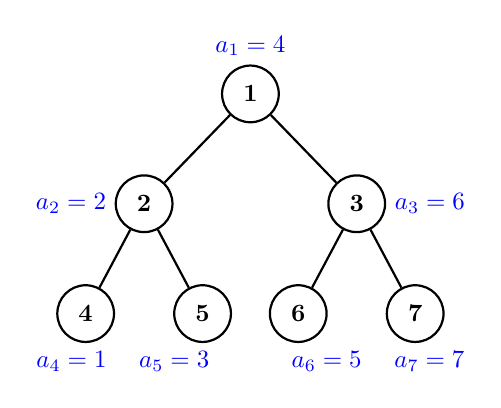
\begin{tikzpicture}[
scale=0.90,
transform shape,
level 1/.style={sibling distance=3.0cm},
level 2/.style={sibling distance=1.65cm},
level distance=1.55cm,
villager/.style={
circle,
draw=black,
thick,
minimum size=0.8cm,
font=\bfseries
},
edge from parent/.style={draw=black, thick}
]
\node[villager, label={[text=blue]above:$a_1=4$}] {1}
child {
node[villager, label={[text=blue]left:$a_2=2$}] {2}
child {
node[villager,
label={[text=blue,xshift=-2mm]below:$a_4=1$}] {4}
}
child {
node[villager,
label={[text=blue,xshift=-4mm]below:$a_5=3$}] {5}
}
}
child {
node[villager, label={[text=blue]right:$a_3=6$}] {3}
child {
node[villager,
label={[text=blue,xshift=4mm]below:$a_6=5$}] {6}
}
child {
node[villager,
label={[text=blue,xshift=2mm]below:$a_7=7$}] {7}
}
};
\end{tikzpicture}
\caption{Initial state}
\end{subfigure}\hfill%
% ---------- (b) 执行 J(1,7) 后 ----------
\begin{subfigure}[t]{0.32\linewidth}
\centering
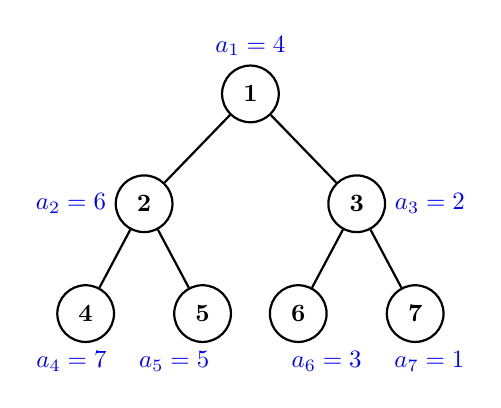
\begin{tikzpicture}[
scale=0.90,
transform shape,
level 1/.style={sibling distance=3.0cm},
level 2/.style={sibling distance=1.65cm},
level distance=1.55cm,
villager/.style={
circle,
draw=black,
thick,
minimum size=0.8cm,
font=\bfseries
},
edge from parent/.style={draw=black, thick}
]
\node[villager, label={[text=blue]above:$a_1=4$}] {1}
child {
node[villager, label={[text=blue]left:$a_2=6$}] {2}
child {
node[villager,
label={[text=blue,xshift=-2mm]below:$a_4=7$}] {4}
}
child {
node[villager,
label={[text=blue,xshift=-4mm]below:$a_5=5$}] {5}
}
}
child {
node[villager, label={[text=blue]right:$a_3=2$}] {3}
child {
node[villager,
label={[text=blue,xshift=4mm]below:$a_6=3$}] {6}
}
child {
node[villager,
label={[text=blue,xshift=2mm]below:$a_7=1$}] {7}
}
};
\end{tikzpicture}
\caption{After Judgment $(1,7)$}
\end{subfigure}\hfill%
% ---------- (c) 再执行 L(4,5) 后 ----------
\begin{subfigure}[t]{0.32\linewidth}
\centering
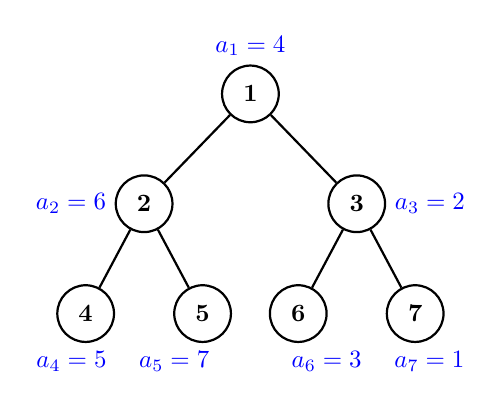
\begin{tikzpicture}[
scale=0.90,
transform shape,
level 1/.style={sibling distance=3.0cm},
level 2/.style={sibling distance=1.65cm},
level distance=1.55cm,
villager/.style={
circle,
draw=black,
thick,
minimum size=0.8cm,
font=\bfseries
},
edge from parent/.style={draw=black, thick}
]
\node[villager, label={[text=blue]above:$a_1=4$}] {1}
child {
node[villager, label={[text=blue]left:$a_2=6$}] {2}
child {
node[villager,
label={[text=blue,xshift=-2mm]below:$a_4=5$}] {4}
}
child {
node[villager,
label={[text=blue,xshift=-4mm]below:$a_5=7$}] {5}
}
}
child {
node[villager, label={[text=blue]right:$a_3=2$}] {3}
child {
node[villager,
label={[text=blue,xshift=4mm]below:$a_6=3$}] {6}
}
child {
node[villager,
label={[text=blue,xshift=2mm]below:$a_7=1$}] {7}
}
};
\end{tikzpicture}
\caption{After Lightning $(4,5)$}
\end{subfigure}

\end{figure}

For the third trident query in the first test case, after the preceding Judgment operation,
the current weights are
\[
(a_1,a_2,\ldots,a_7)=(4,6,2,7,5,3,1).
\]

Weights $4,5,6,7$ are at vertices $1,5,2,4$, respectively, so $S=\{1,2,4,5\}$.

Choose $F=1$, $x=4$, and $y=5$. Then:

\begin{itemize}
\item Vertex $1$ is an ancestor of vertex $4$.
\item Vertex $1$ is an ancestor of vertex $5$.
\item $ P(1,4)\cup P(1,5) =\{1,2,4\}\cup\{1,2,5\}=S$。
\end{itemize}

Therefore, $S$ is a \textbf{trident}.


